\newcolumntype{M}[1]{>{\centering\arraybackslash}m{#1}}
\begin{figure}[p!] % Place the grid on a separate page
\centering
\begin{tabular}{@{} M{0.166\textwidth} M{0.166\textwidth} | M{0.166\textwidth} M{0.166\textwidth} | M{0.166\textwidth} M{0.166\textwidth} @{}}
       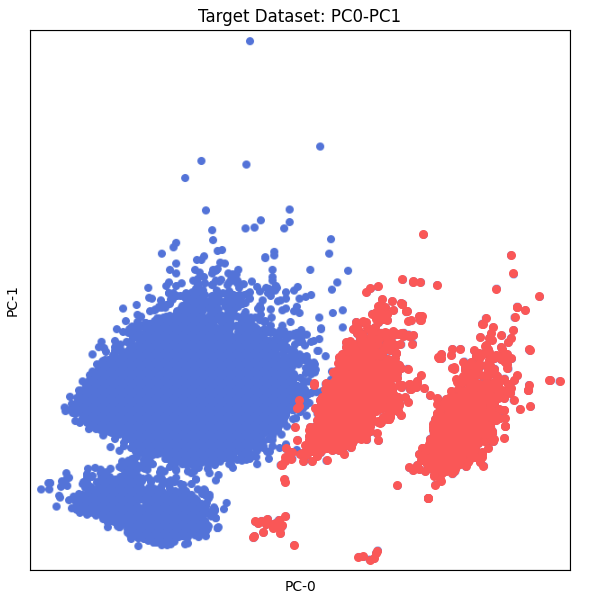
\includegraphics[width=\linewidth]{z_Sample40.orig.png} &
       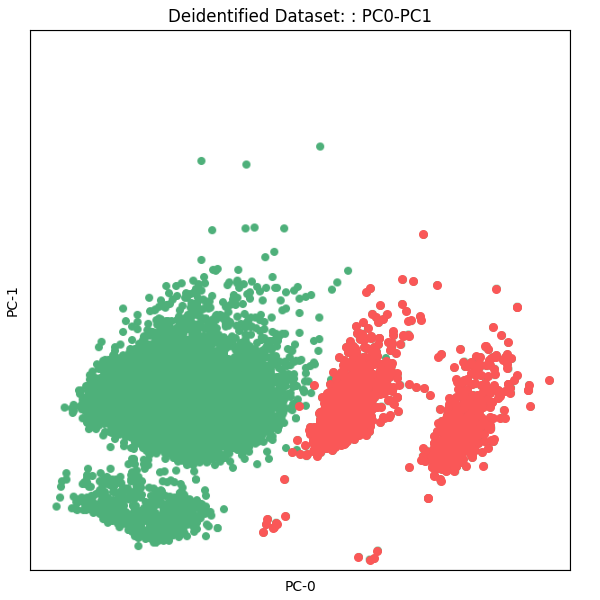
\includegraphics[width=\linewidth]{z_Sample40.syn.png} &
       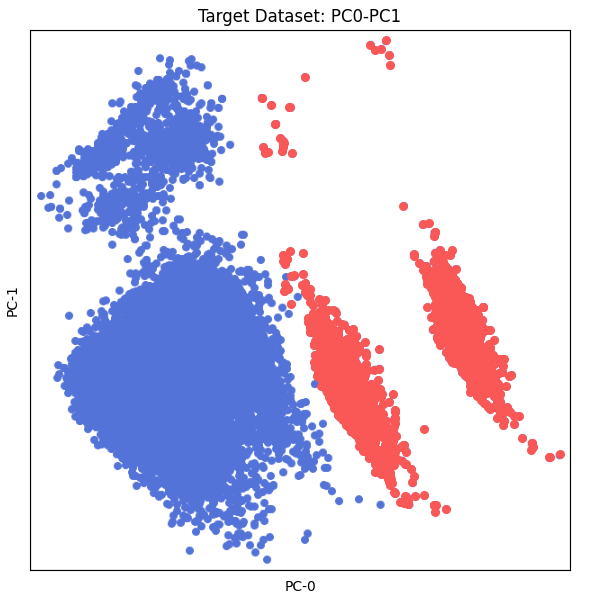
\includegraphics[width=\linewidth]{z_CART.orig.png} &
       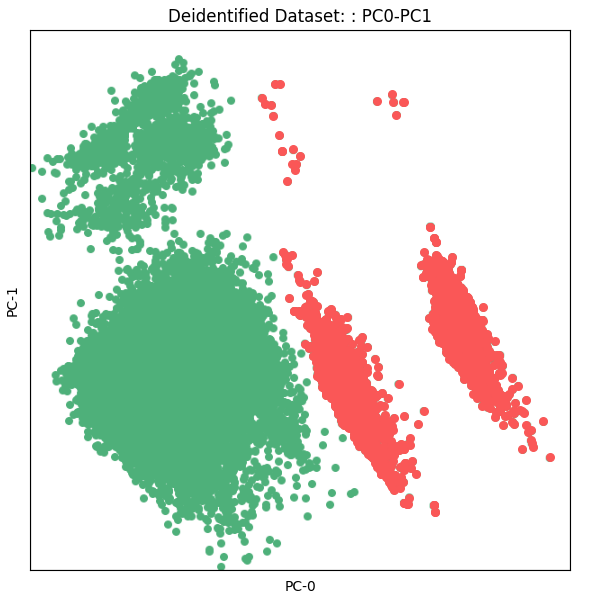
\includegraphics[width=\linewidth]{z_CART.syn.png} &
       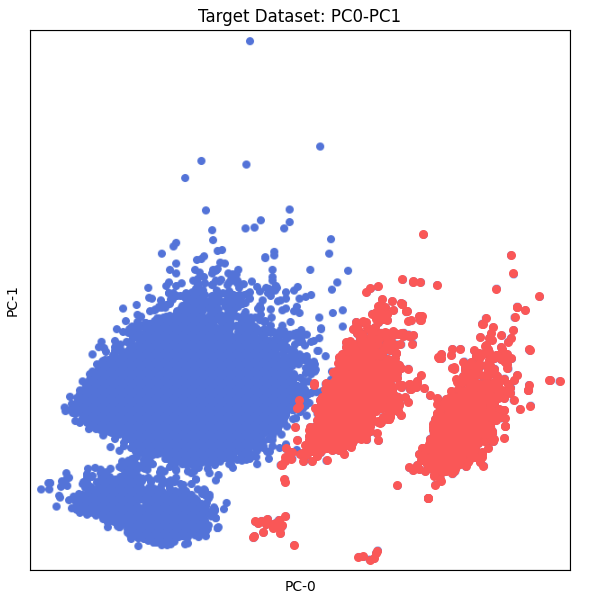
\includegraphics[width=\linewidth]{z_Aindo.orig.png} &
       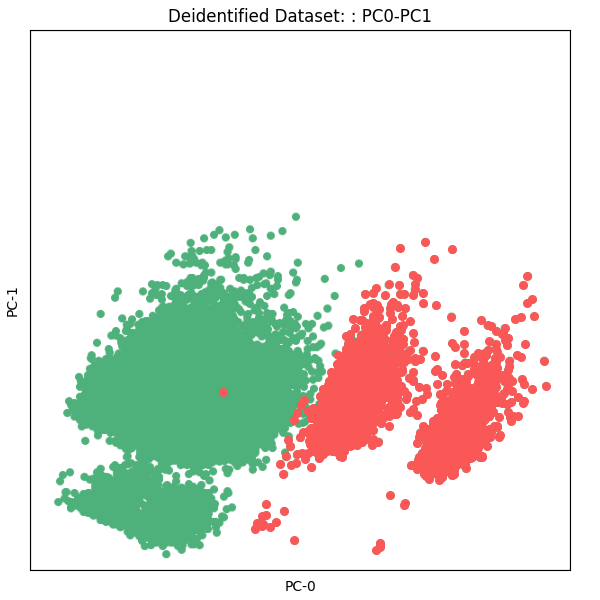
\includegraphics[width=\linewidth]{z_Aindo.syn.png} \\ 
\multicolumn{2}{c|}{Sample40, 0.0055} &
\multicolumn{2}{c|}{CART, 0.0068} &
\multicolumn{2}{c}{Aindo, 0.0089} \\ 
 \hline 
       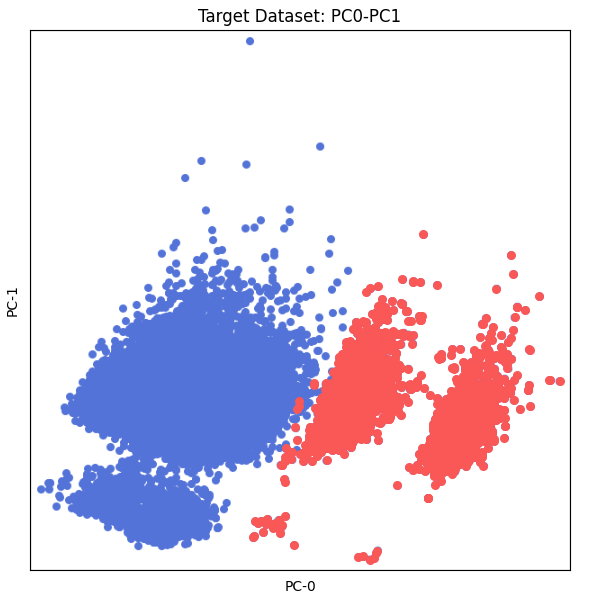
\includegraphics[width=\linewidth]{z_Anonos.orig.png} &
       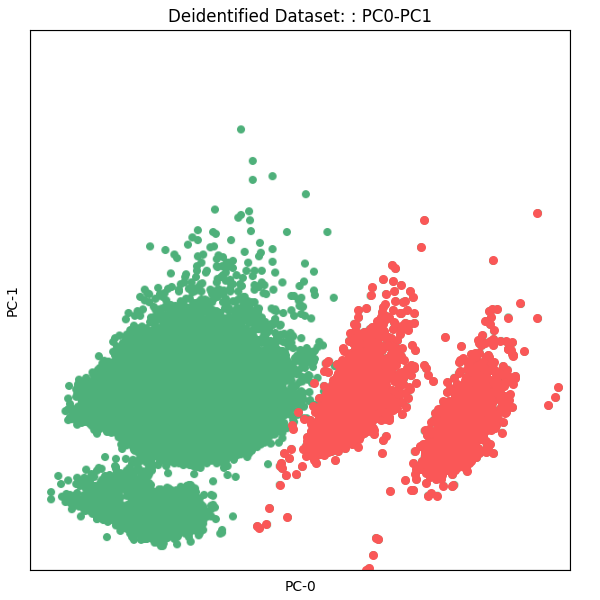
\includegraphics[width=\linewidth]{z_Anonos.syn.png} &
       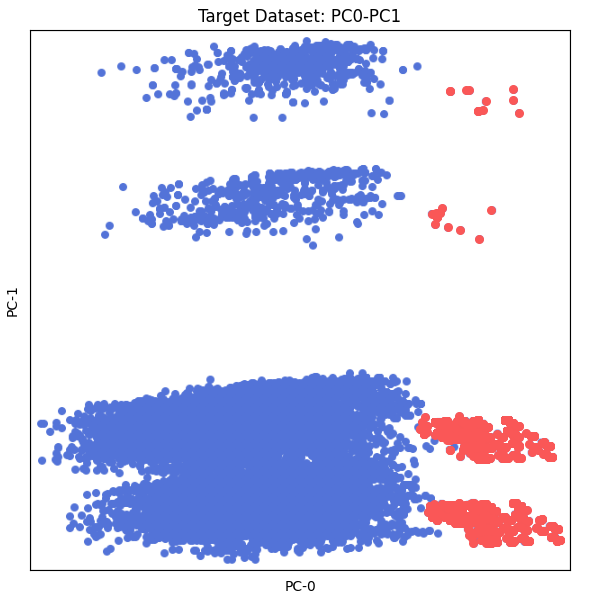
\includegraphics[width=\linewidth]{z_PRAM.orig.png} &
       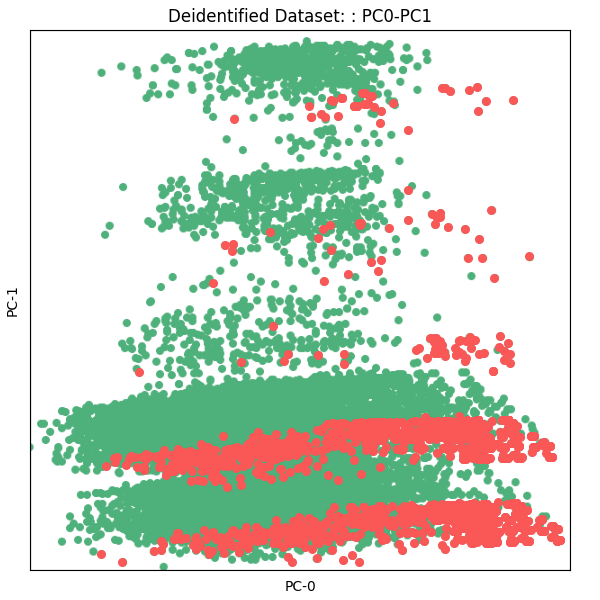
\includegraphics[width=\linewidth]{z_PRAM.syn.png} &
       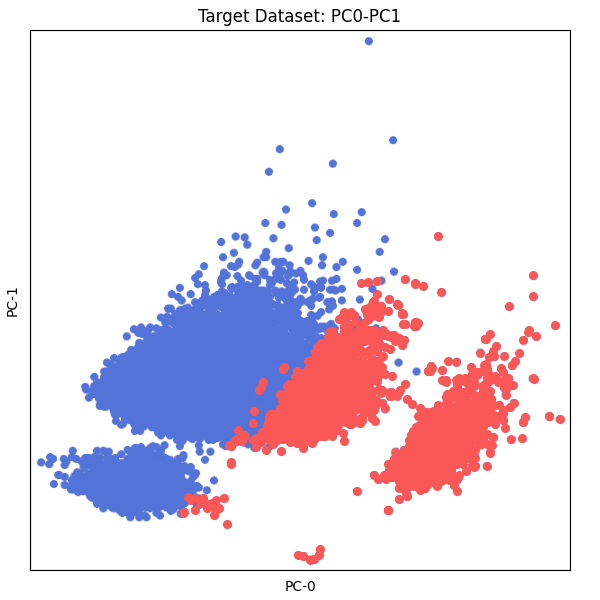
\includegraphics[width=\linewidth]{z_MostlyAI.orig.png} &
       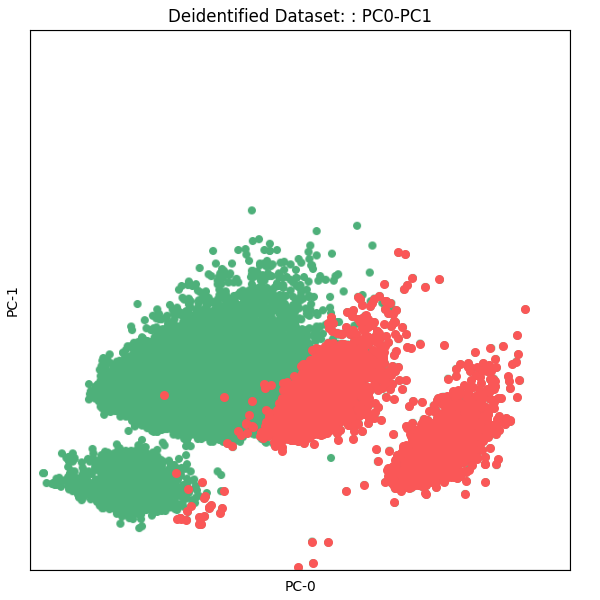
\includegraphics[width=\linewidth]{z_MostlyAI.syn.png} \\ 
\multicolumn{2}{c|}{Anonos, 0.0106} &
\multicolumn{2}{c|}{PRAM, 0.0144} &
\multicolumn{2}{c}{MostlyAI, 0.0166} \\ 
 \hline 
       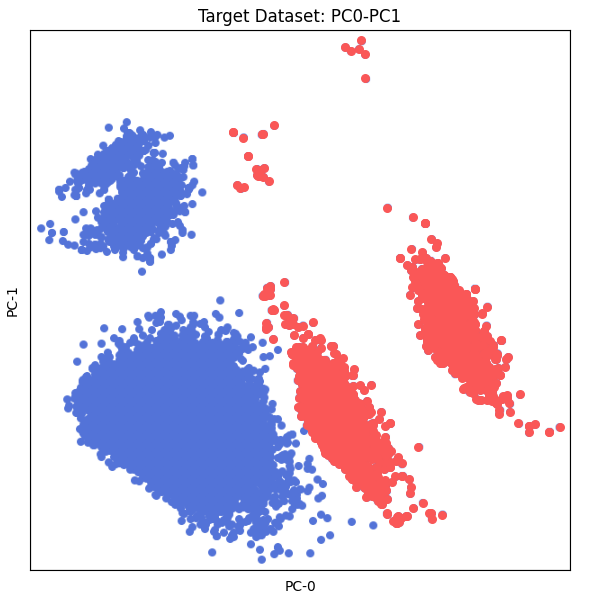
\includegraphics[width=\linewidth]{z_Genetic.orig.png} &
       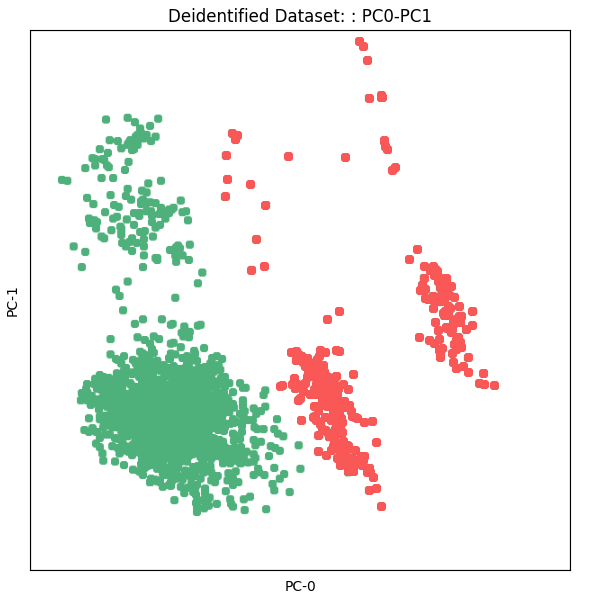
\includegraphics[width=\linewidth]{z_Genetic.syn.png} &
       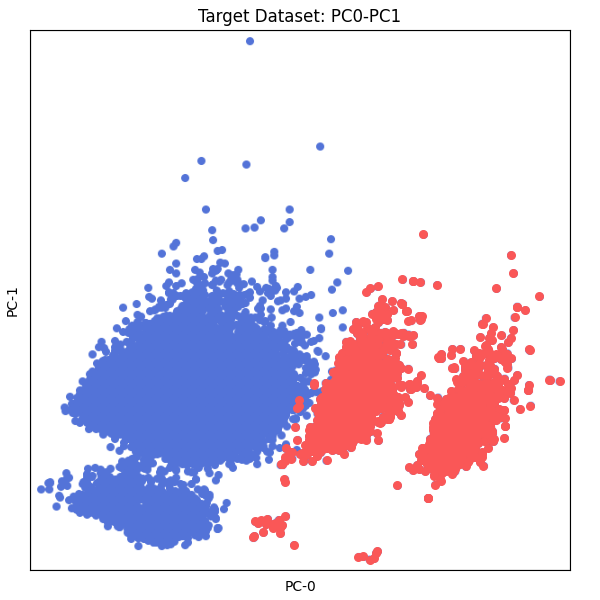
\includegraphics[width=\linewidth]{z_SynDiffix.orig.png} &
       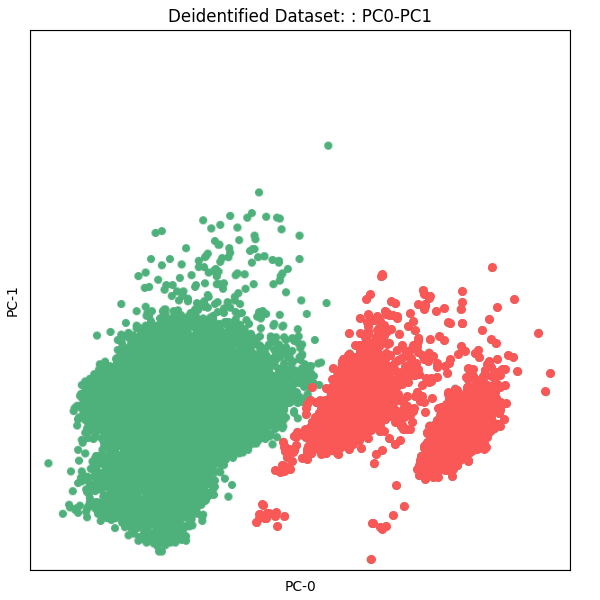
\includegraphics[width=\linewidth]{z_SynDiffix.syn.png} &
       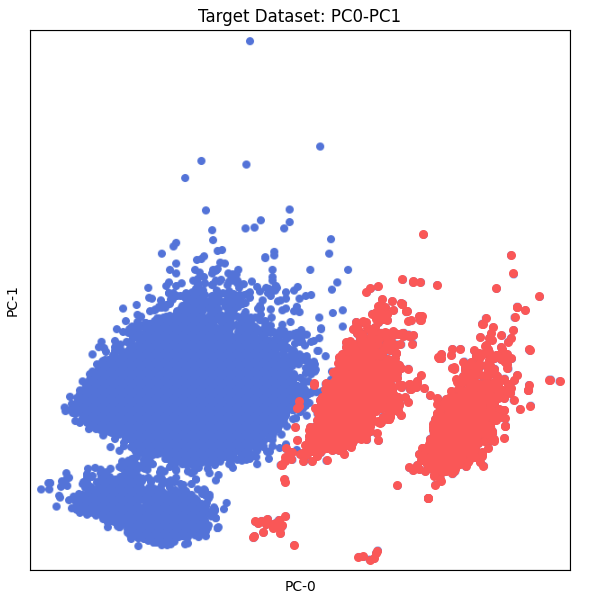
\includegraphics[width=\linewidth]{z_sdx-single.orig.png} &
       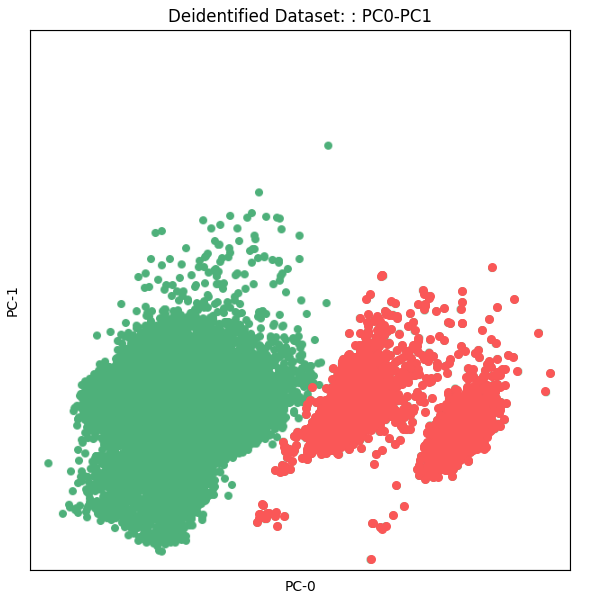
\includegraphics[width=\linewidth]{z_sdx-single.syn.png} \\ 
\multicolumn{2}{c|}{Genetic, 0.0243} &
\multicolumn{2}{c|}{SynDiffix, 0.0272} &
\multicolumn{2}{c}{sdx-single, 0.0272} \\ 
 \hline 
       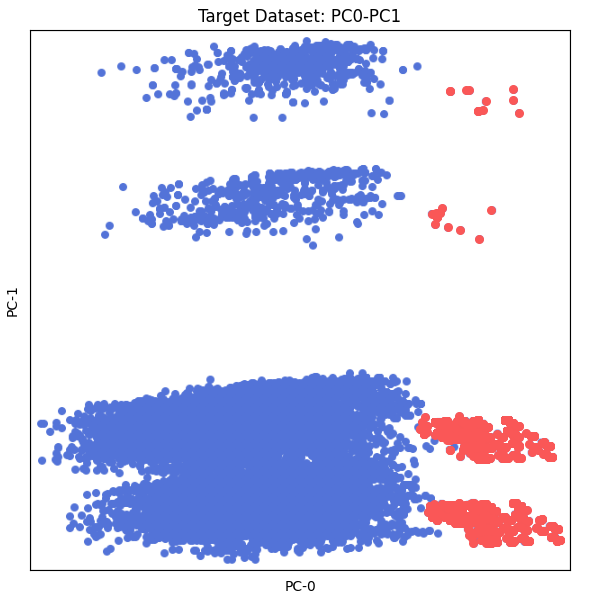
\includegraphics[width=\linewidth]{z_Sarus.orig.png} &
       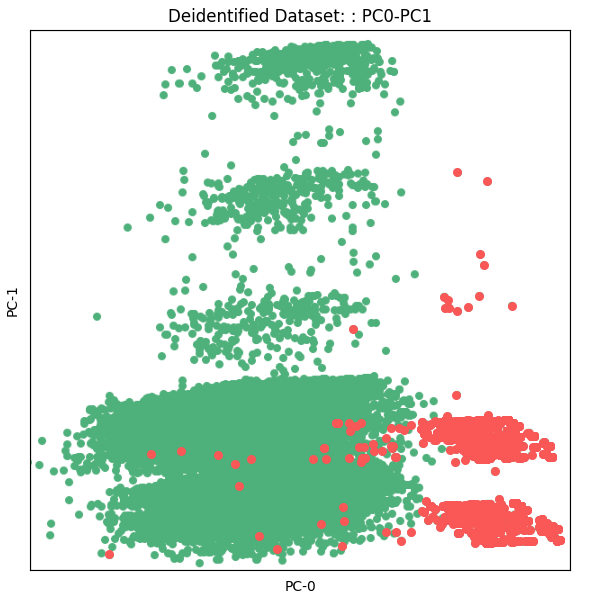
\includegraphics[width=\linewidth]{z_Sarus.syn.png} &
       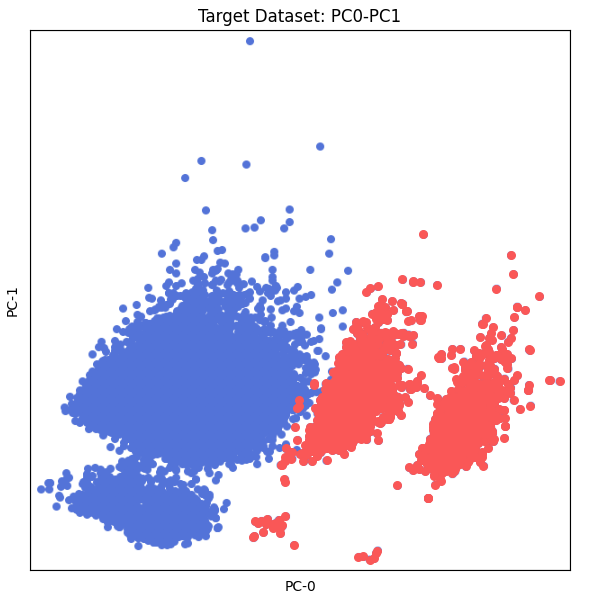
\includegraphics[width=\linewidth]{z_AIM.orig.png} &
       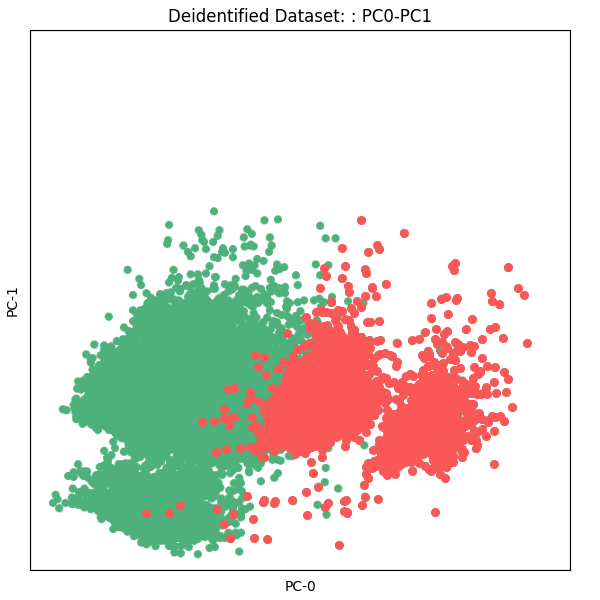
\includegraphics[width=\linewidth]{z_AIM.syn.png} &
       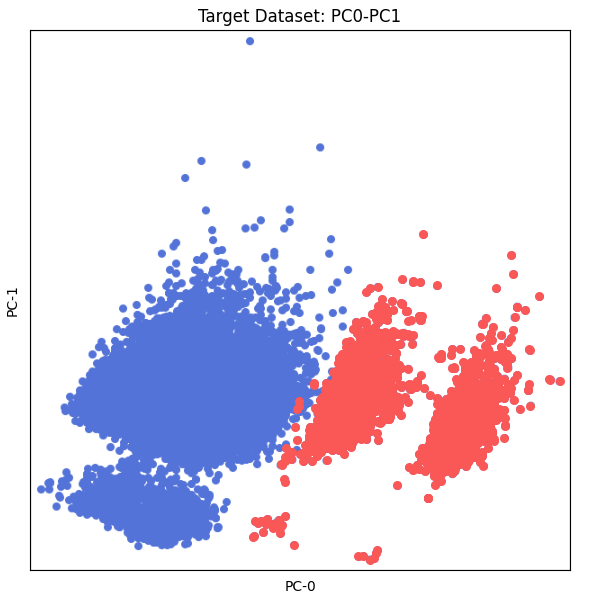
\includegraphics[width=\linewidth]{z_CTGAN.orig.png} &
       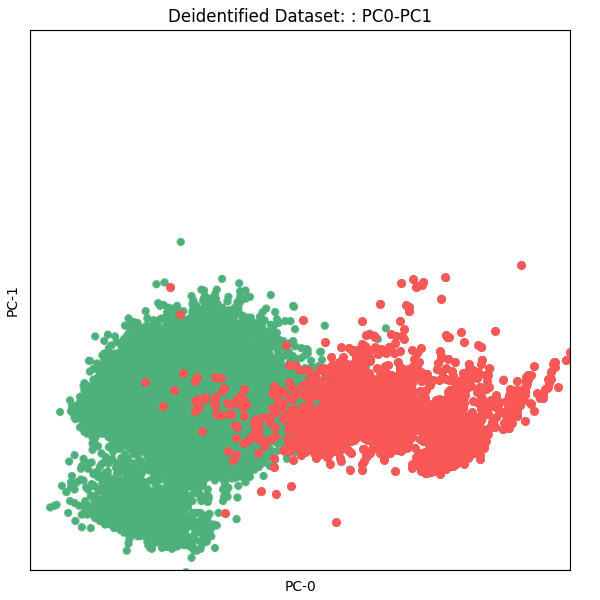
\includegraphics[width=\linewidth]{z_CTGAN.syn.png} \\ 
\multicolumn{2}{c|}{Sarus, 0.0317} &
\multicolumn{2}{c|}{AIM, 0.0391} &
\multicolumn{2}{c}{CTGAN, 0.0394} \\ 
 \hline 
       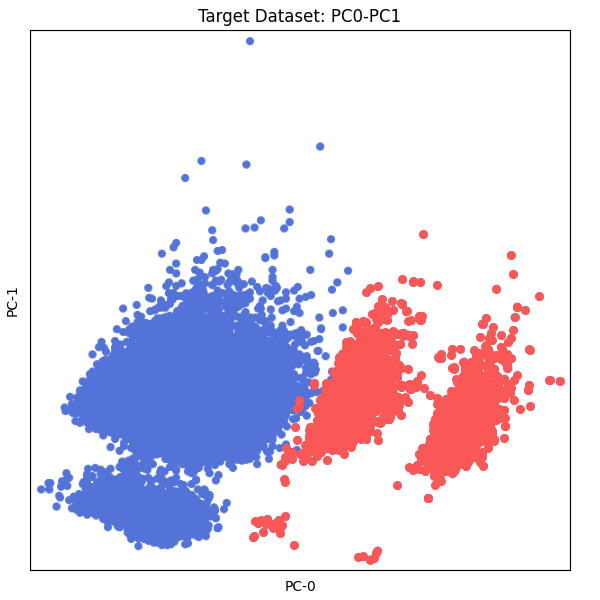
\includegraphics[width=\linewidth]{z_mwem-pgm.orig.png} &
       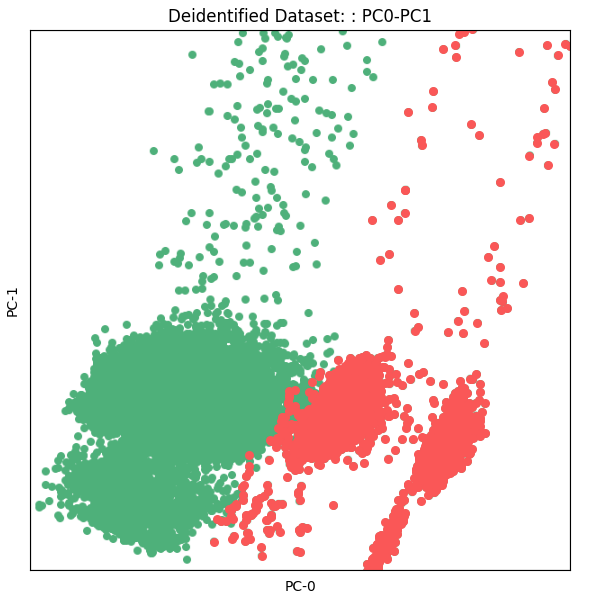
\includegraphics[width=\linewidth]{z_mwem-pgm.syn.png} &
       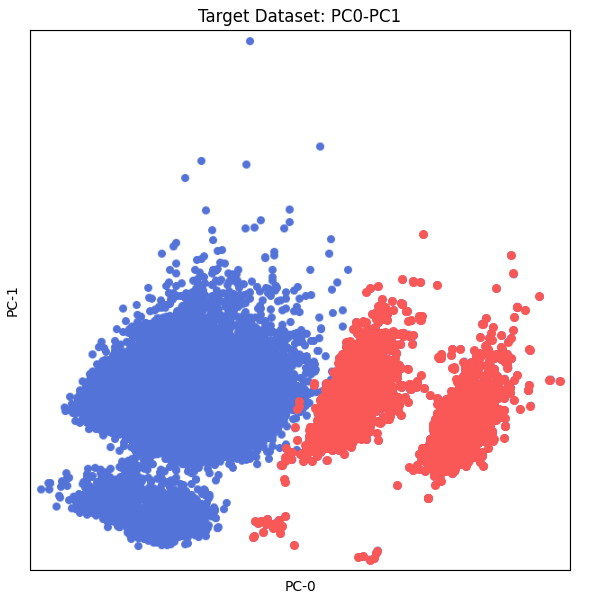
\includegraphics[width=\linewidth]{z_YData.orig.png} &
       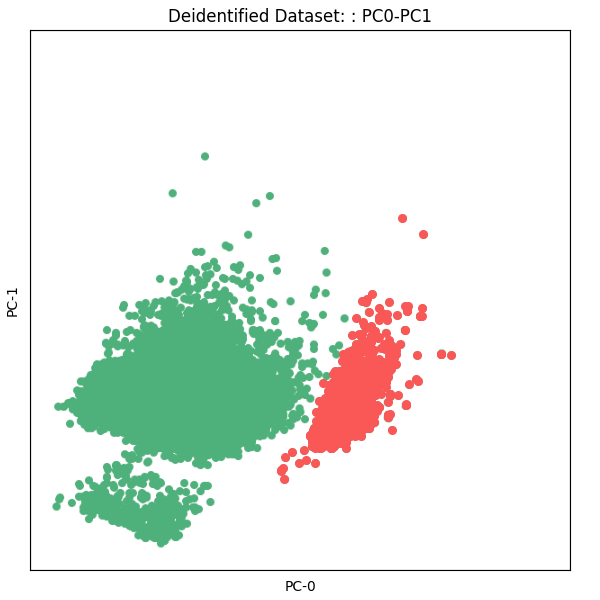
\includegraphics[width=\linewidth]{z_YData.syn.png} &
       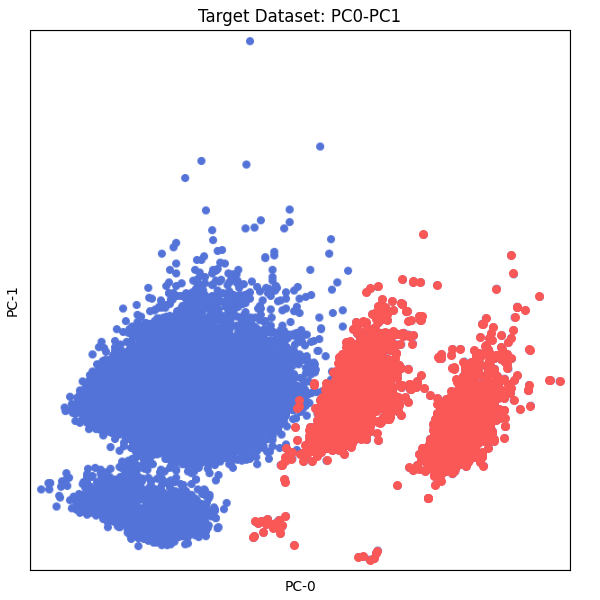
\includegraphics[width=\linewidth]{z_SMOTE.orig.png} &
       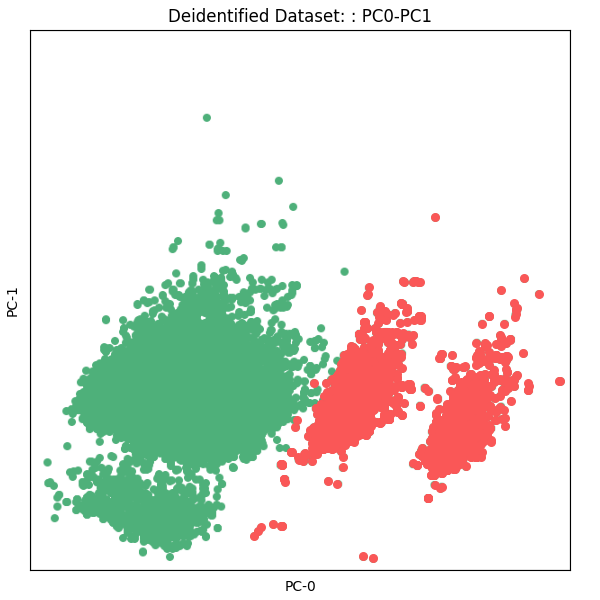
\includegraphics[width=\linewidth]{z_SMOTE.syn.png} \\ 
\multicolumn{2}{c|}{mwem-pgm, 0.0458} &
\multicolumn{2}{c|}{YData, 0.0518} &
\multicolumn{2}{c}{SMOTE, 0.0518} \\ 
 \hline 
       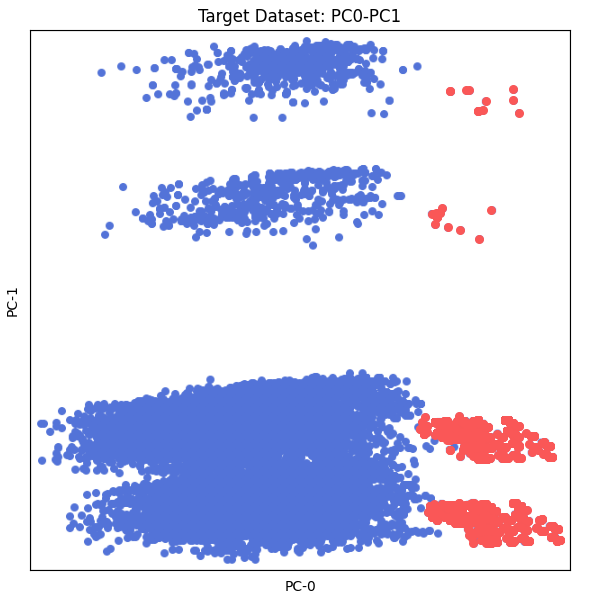
\includegraphics[width=\linewidth]{z_K6-Anon.orig.png} &
       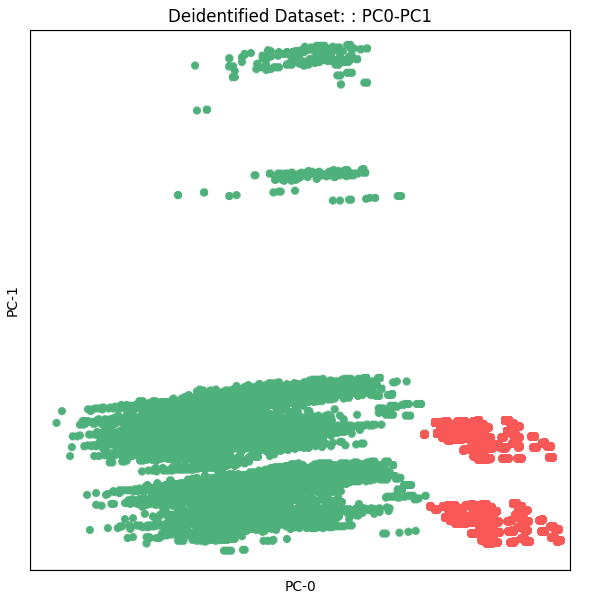
\includegraphics[width=\linewidth]{z_K6-Anon.syn.png} &
       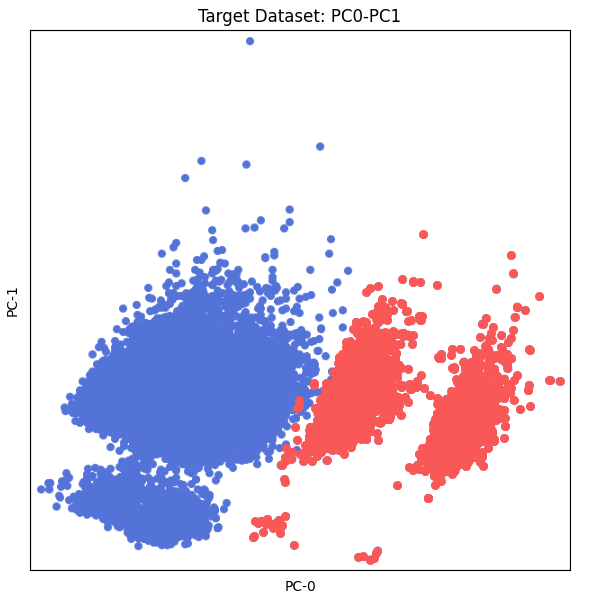
\includegraphics[width=\linewidth]{z_Pategan.orig.png} &
       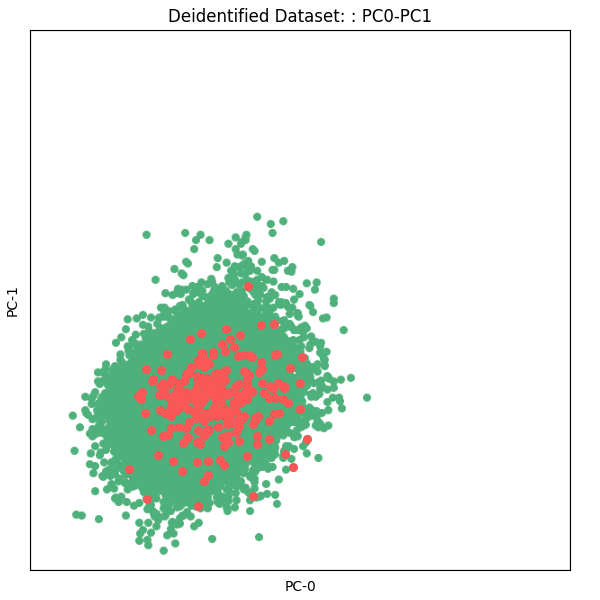
\includegraphics[width=\linewidth]{z_Pategan.syn.png} \\ 
\multicolumn{2}{c|}{K6-Anon, 0.0619} &
\multicolumn{2}{c}{Pategan, 0.1402} \\ 
    \end{tabular}
\caption{Original (left) and synthetic (right) scatterplot and average Kolmogorov-Smirnov score for all principle components, ordered by most-to-least accurate.}
\label{fig:pca_grid}
\end{figure}